% !TEX root = ../main.tex
% !TEX spellcheck = en_GB

\chapter{Results}
\label{chap:results}
This chapter compares the created models with the measurements.

Figures~\ref{fig:allcompareseethrough} and \ref{fig:allcomparewooden} shows the comparisons of the drive unit model, cabinet model and the measurements of the see-through and wooden speakers.
As can be seen, the cabinet model is way off, suggesting that the two cabinets were not air tight during the measurements.
The drive unit model does seem to follow the measurement, as the two seem to flatten out at around the same spot.
The reason for the models to have a slightly higher amplitude, is probably due to some losses, which the model has not taken into account.

\fxnote{Måske billede af fountek driver data sheet frekvenskarakteristik?}

\begin{figure}
	\centering
	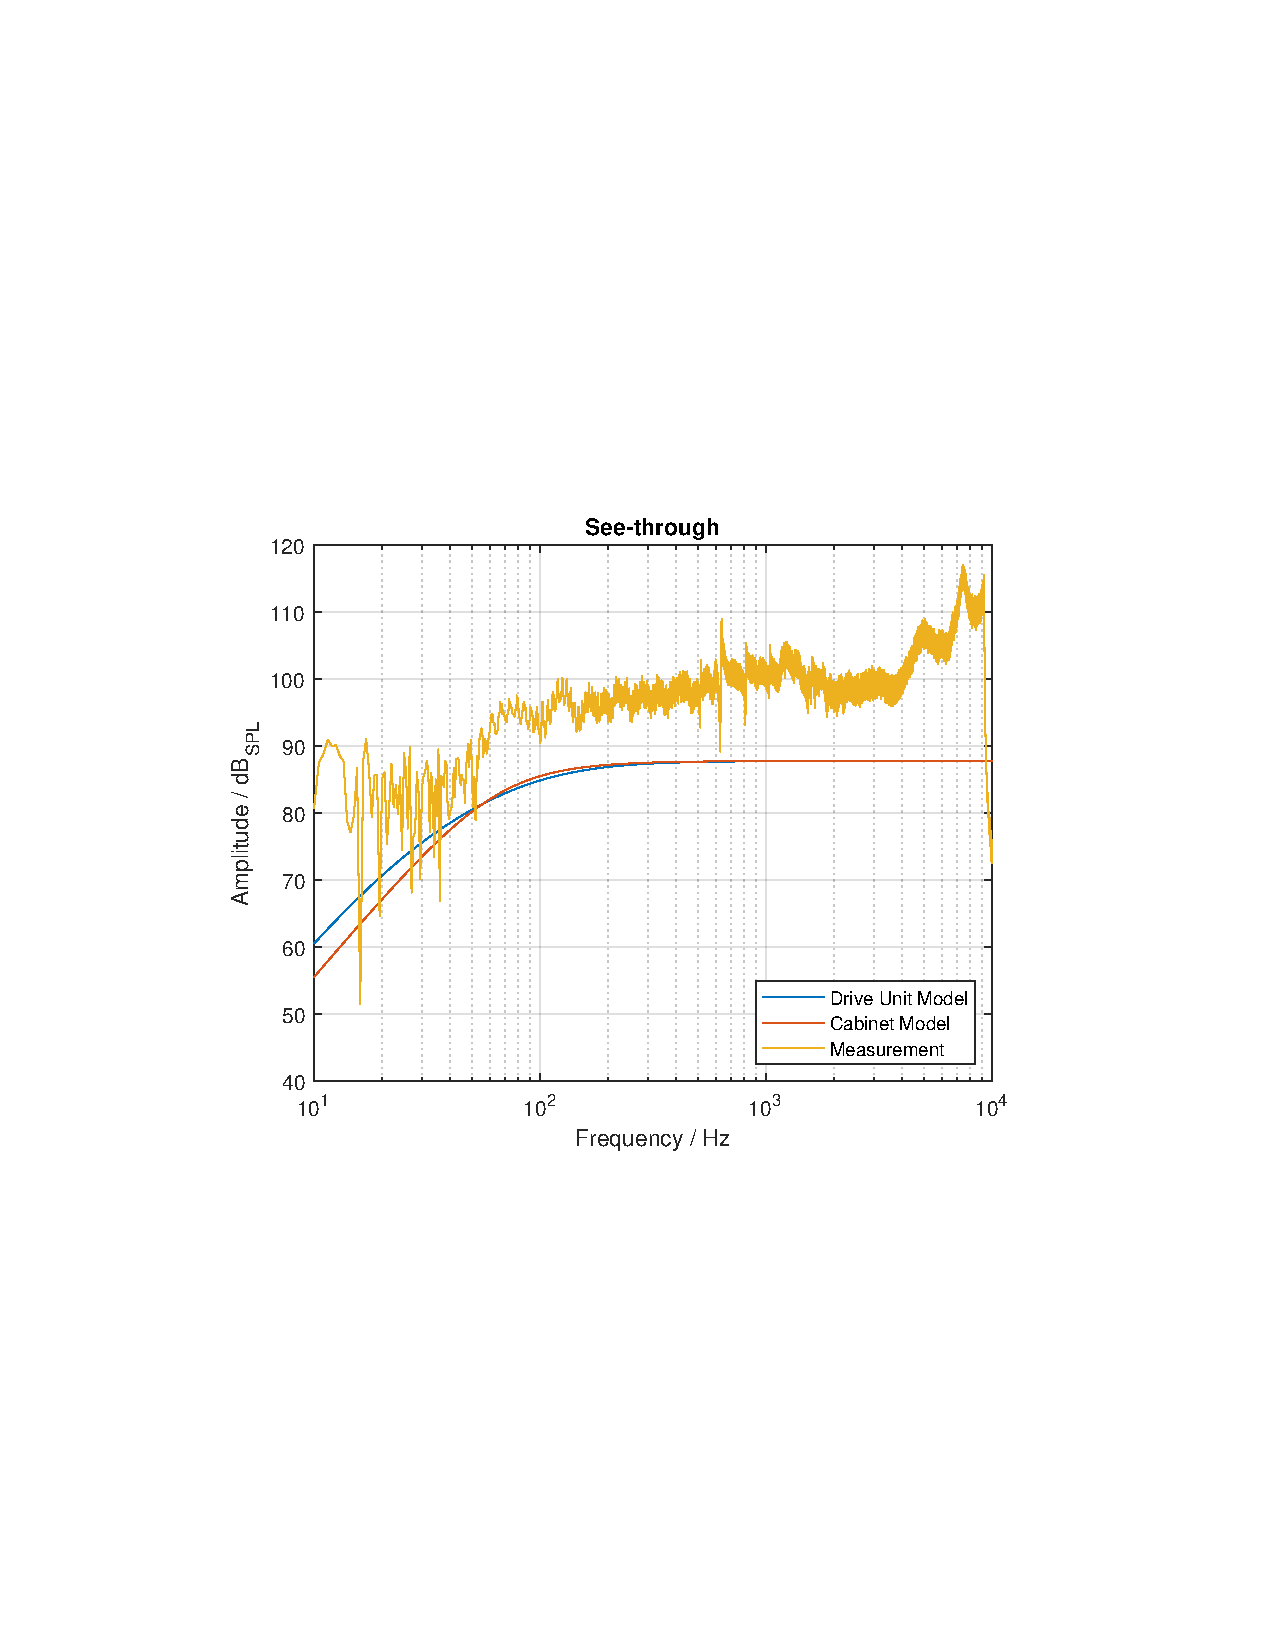
\includegraphics[width=0.7\linewidth, clip, trim={3.9cm 8.4cm 4.5cm 8.5cm}]{gfx/Results/AllCompareSeeThrough.pdf}
	\caption{The two models for the Drive Unit (blue), Cabinet (red) and the measurement of the see-through speaker (orange).}
	\label{fig:allcompareseethrough}
\end{figure}

\begin{figure}
	\centering
	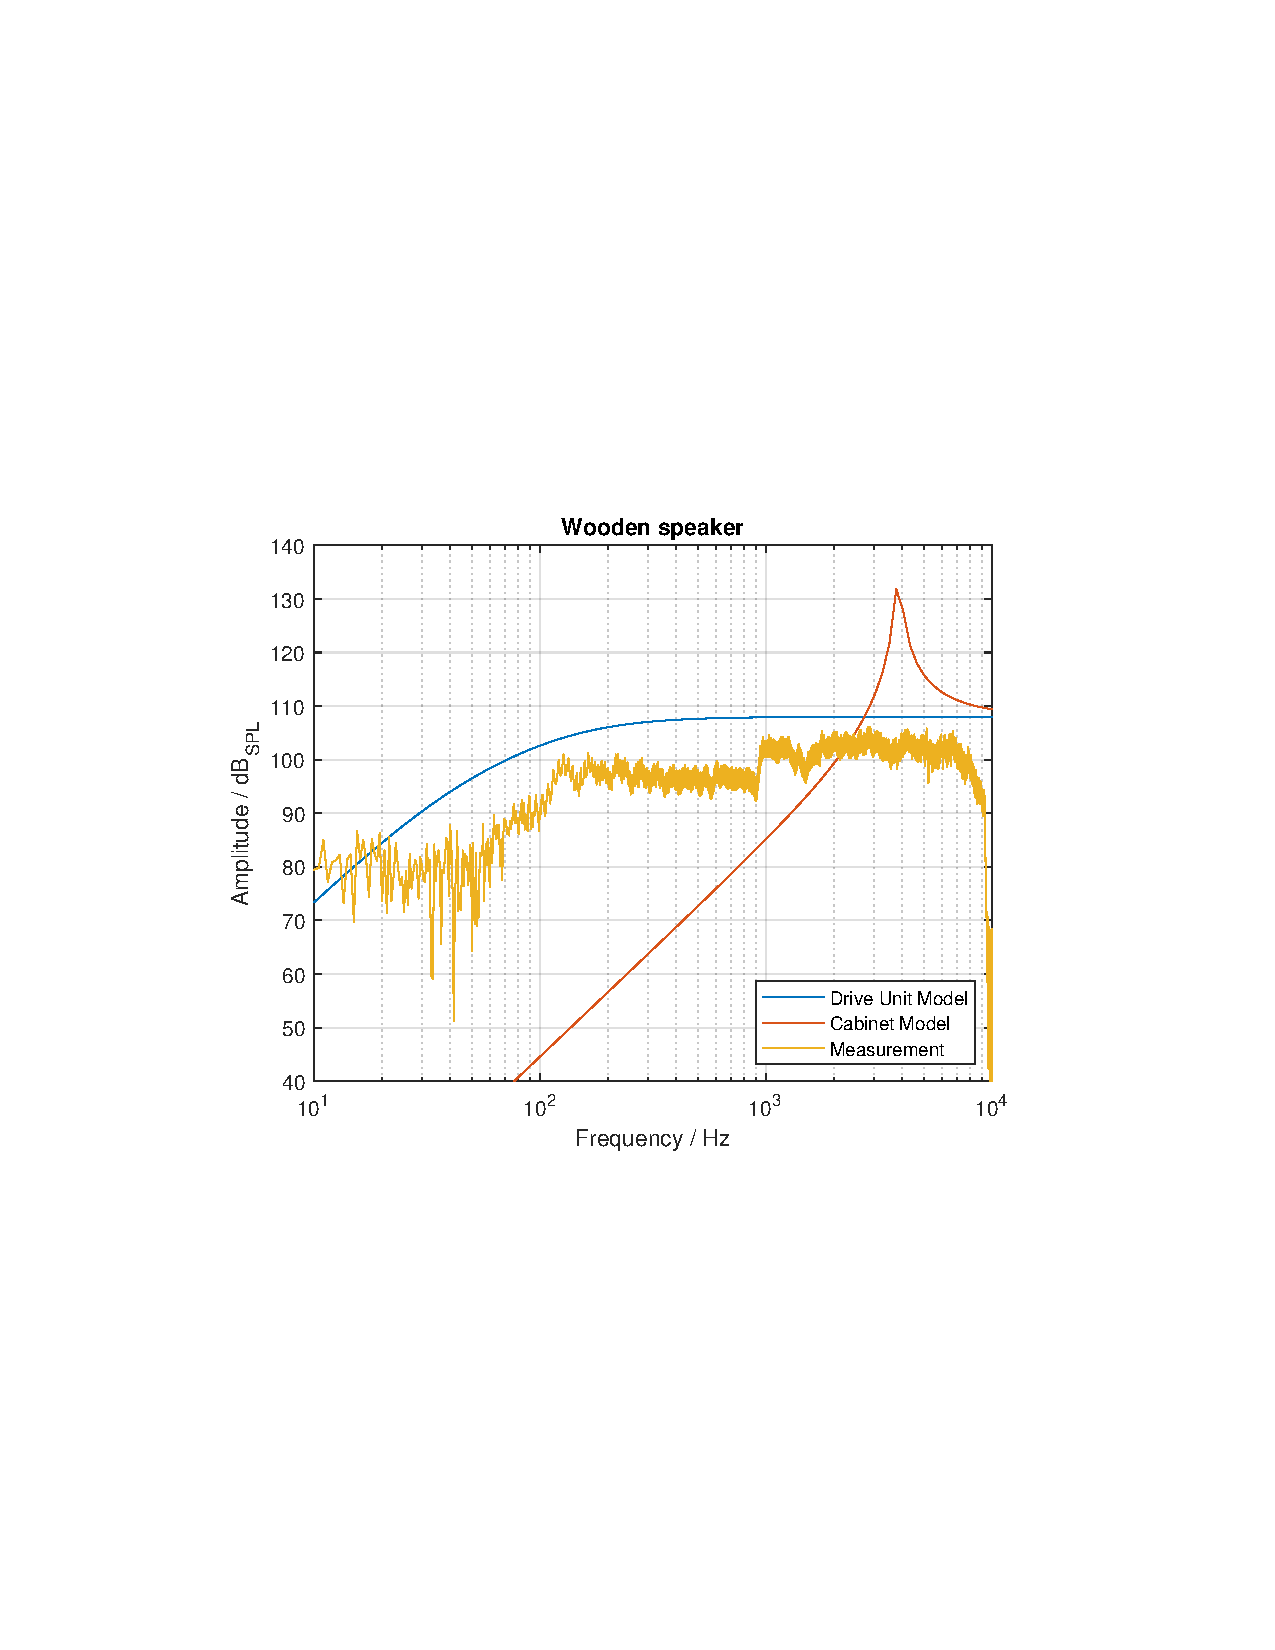
\includegraphics[width=0.7\linewidth, clip, trim={3.9cm 8.4cm 4.5cm 8.5cm}]{gfx/Results/AllCompareWooden.pdf}
	\caption{The two models for the Drive Unit (blue), Cabinet (red) and the measurement of the wooden speaker (orange).}
	\label{fig:allcomparewooden}
\end{figure}

\fxnote{Compare: DUmodel(ST, wood) with meas(ST, wood). Show CABmodel and say not alike.}
\fxnote{Compare \cref{fig:PGcompareAll} with expected effect of bass reflex}
\fxnote{Resonance freq. p. 55 TAS}
\FloatBarrier